\documentclass[11pt]{article}
\usepackage{graphicx}
\usepackage{booktabs}
\usepackage{amsmath}
\usepackage[hidelinks]{hyperref}
\usepackage{geometry}
\usepackage{caption}
\geometry{margin=1in}
\captionsetup{font=small,labelfont=bf}

\title{Predictors of Student Academic Performance:\\
A Regression-Based Analysis of Effort, Background, and Outcome}
\author{Researcher Skill (auto-generated)}
\date{\today}

\begin{document}
\maketitle

\begin{abstract}
We analyze a dataset of 500 secondary-school students containing behavioral, demographic, and academic outcome variables to identify which factors most strongly predict final academic score. A multiple linear regression on nine candidate predictors explains 76.7\% of the variance in final score ($R^2=0.767$, Adj.\ $R^2=0.763$, $\text{RMSE}=7.49$). Weekly study hours dominates all other predictors (standardized $\beta=+0.83$, $p<10^{-100}$), followed by attendance rate ($\beta=+0.26$) and previous score ($\beta=+0.24$). Demographic and contextual variables---gender, age, parental education, internet access, and extracurricular participation---are not statistically significant after controlling for effort. A logistic pass/fail model achieves 84.4\% accuracy against a 64.6\% base rate. Students in the top study-hours tertile pass at dramatically higher rates than those in the bottom tertile. The results suggest that interventions targeting study habits and attendance are the highest-leverage levers for improving student outcomes in this population.
\end{abstract}

\section{Introduction}
Understanding what drives academic performance is a perennial question in education research. Two broad families of explanation compete: \emph{effort-based} accounts, which emphasize study behaviors such as time on task and attendance; and \emph{contextual} accounts, which emphasize demographic background, parental education, and access to resources. Both families receive empirical support in the literature, but their relative importance varies substantially across samples and settings.

This paper uses a dataset of 500 students with paired behavioral, demographic, and outcome variables to address the following research question:

\begin{quote}\itshape
Which factors---study hours, attendance, prior performance, parental education, internet access, and extracurricular participation---are the strongest predictors of a student's final score, and how much of the variance can they jointly explain?
\end{quote}

Two supporting questions are considered: (i) what combination of variables best discriminates students who pass from those who fail; and (ii) whether demographic factors create achievement gaps after controlling for effort variables.

\section{Data}
The dataset \texttt{student\_performance.csv} contains 500 student records with 11 variables (Table~\ref{tab:vars}). Each record includes demographic attributes (gender, age), parental education, behavioral measures (weekly study hours, attendance rate, extracurricular participation, internet access), an indicator of prior academic standing (\texttt{previous\_score}), and two outcome variables (\texttt{final\_score} and a binary \texttt{passed} flag).

\begin{table}[htbp]
\centering
\small
\caption{Variables in the dataset.}
\label{tab:vars}
\begin{tabular}{lll}
\toprule
Variable & Type & Summary \\
\midrule
\texttt{student\_id}             & ID         & 500 unique \\
\texttt{gender}                  & categorical & Female 54.6\%, Male 45.4\% \\
\texttt{age}                     & integer    & range 15--19, mean 16.98 \\
\texttt{study\_hours\_per\_week} & integer    & range 2--30, mean 15.31 \\
\texttt{attendance\_rate}        & float (\%) & range 50.2--100, mean 76.38 \\
\texttt{parent\_education}       & categorical & 4 levels; 23.4\% missing \\
\texttt{internet\_access}        & binary     & Yes 50.8\%, No 49.2\% \\
\texttt{extracurricular}         & binary     & Yes 49.4\%, No 50.6\% \\
\texttt{previous\_score}         & integer    & range 30--95, mean 62.99 \\
\texttt{final\_score}            & integer    & range 20--95, mean 55.98 \\
\texttt{passed}                  & binary     & Yes 64.6\%, No 35.4\% \\
\bottomrule
\end{tabular}
\end{table}

Missing values occur only in \texttt{parent\_education} (117/500, 23.4\%). For modeling, the variable was ordinal-encoded (None=0, High School=1, Bachelor=2, Master=3, PhD=4) and missing values imputed with the median, with an auxiliary binary \texttt{parent\_edu\_missing} indicator added to the design matrix. Binary categorical variables were 0/1 encoded.

Figure~\ref{fig:dist} shows the distribution of numeric variables. Final score is approximately symmetric and spans the full 20--95 range.

\begin{figure}[htbp]
  \centering
  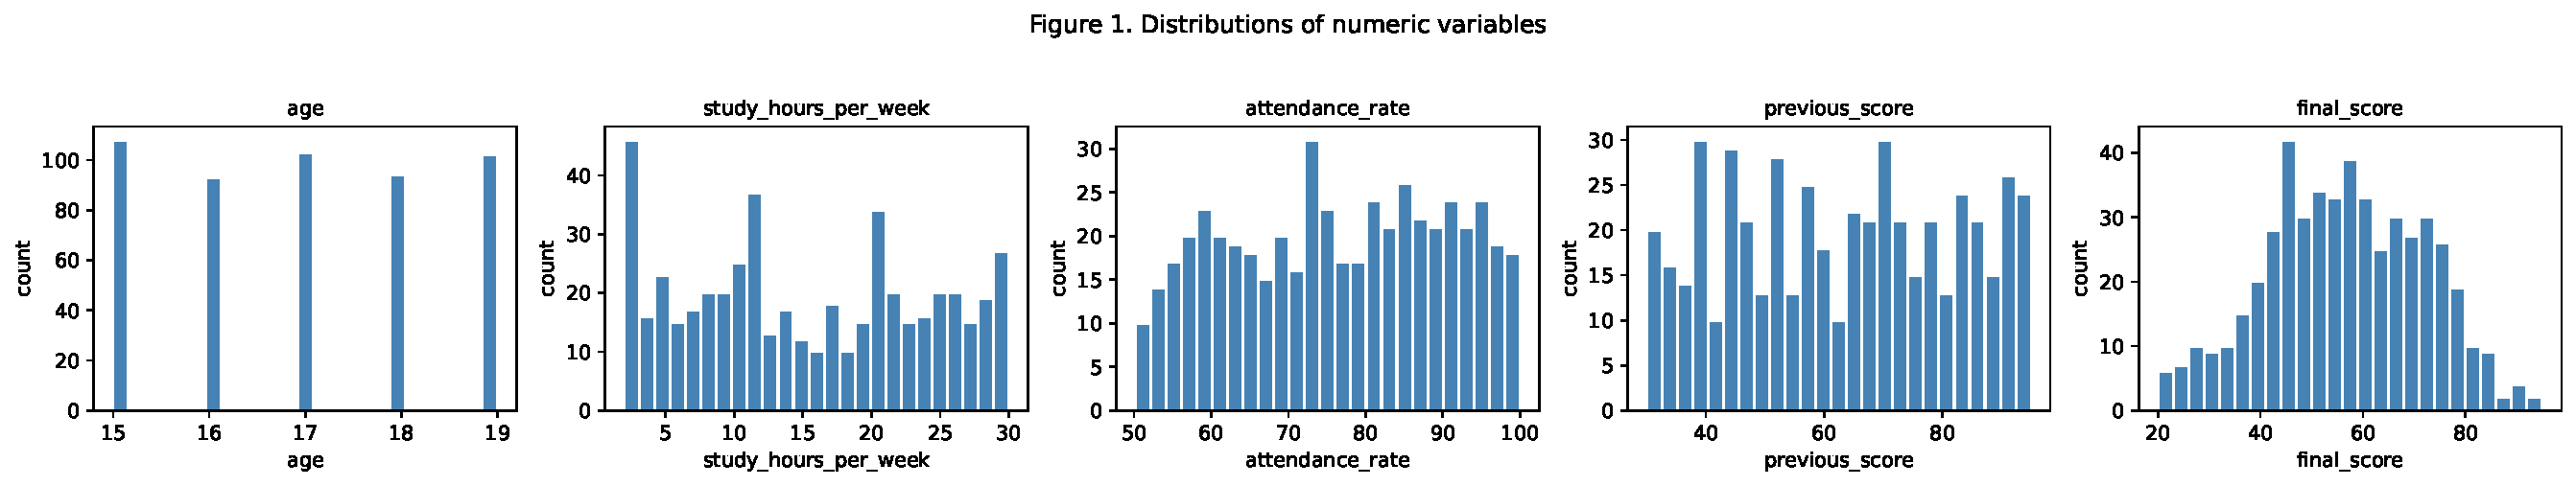
\includegraphics[width=\textwidth]{fig1_distributions.pdf}
  \caption{Distributions of numeric variables.}
  \label{fig:dist}
\end{figure}

\section{Methodology}
We conducted four complementary analyses:

\begin{enumerate}
  \item \textbf{Univariate summaries} of each variable (means, standard deviations, counts).
  \item \textbf{Pearson correlations} between each numeric/binary predictor and \texttt{final\_score}.
  \item \textbf{Ordinary least squares (OLS) multiple regression} of \texttt{final\_score} on nine predictors: study hours per week, attendance rate, previous score, age, female indicator, internet access, extracurricular, parental education ordinal, and missingness indicator.
  \item \textbf{Logistic regression} of the binary \texttt{passed} outcome on the same predictor set, fit via iteratively re-weighted least squares (IRLS), with classification accuracy reported at the 0.5 threshold.
\end{enumerate}

Group comparisons (Welch's $t$-test for binary factors; one-way ANOVA for parental education) were additionally performed to test for univariate differences in final score. All analyses were implemented in Python using only \texttt{numpy}, \texttt{pandas}, and \texttt{matplotlib}; see the accompanying Jupyter notebook \texttt{research\_notebook.ipynb} for a fully reproducible pipeline.

\section{Results}

\subsection{Correlations with final score}
Table~\ref{tab:corr} reports Pearson correlations between each predictor and the final score. Study hours per week shows a very strong positive correlation ($r=+0.80$), attendance rate a moderate correlation ($r=+0.24$), and previous score a weaker but statistically significant correlation ($r=+0.17$). All demographic and contextual predictors show correlations near zero.

\begin{table}[htbp]
\centering
\small
\caption{Pearson correlations with \texttt{final\_score}.}
\label{tab:corr}
\begin{tabular}{lrr}
\toprule
Variable & $r$ & $p$ \\
\midrule
study\_hours\_per\_week   & $+0.804$ & $<10^{-100}$ \\
attendance\_rate          & $+0.241$ & $5.1\times10^{-8}$ \\
previous\_score           & $+0.165$ & $2.1\times10^{-4}$ \\
internet\_access (=Yes)   & $+0.051$ & $0.259$ \\
age                       & $-0.048$ & $0.286$ \\
parent\_edu (ordinal)     & $+0.044$ & $0.390$ \\
gender (=Female)          & $-0.031$ & $0.485$ \\
extracurricular (=Yes)    & $+0.029$ & $0.519$ \\
\bottomrule
\end{tabular}
\end{table}

\begin{figure}[htbp]
  \centering
  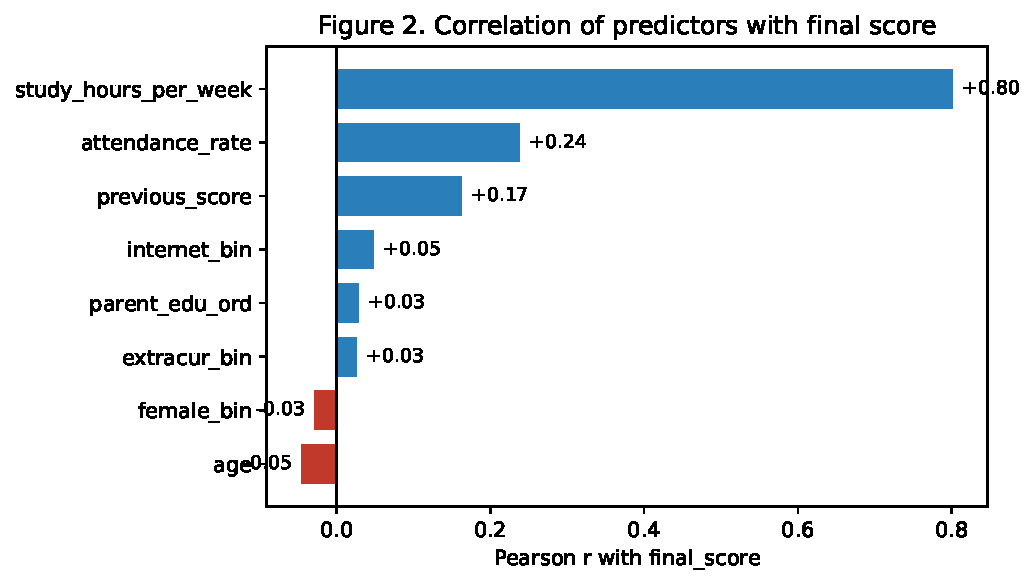
\includegraphics[width=0.85\textwidth]{fig2_correlations.pdf}
  \caption{Pearson correlations of each predictor with final score. Blue bars are positive, red bars negative.}
  \label{fig:corr}
\end{figure}

\subsection{Study hours and final score}
Figure~\ref{fig:hours} shows the bivariate relationship between study hours and final score, coloured by pass/fail. The linear fit has a slope of approximately $+1.49$ points per additional weekly study hour.

\begin{figure}[htbp]
  \centering
  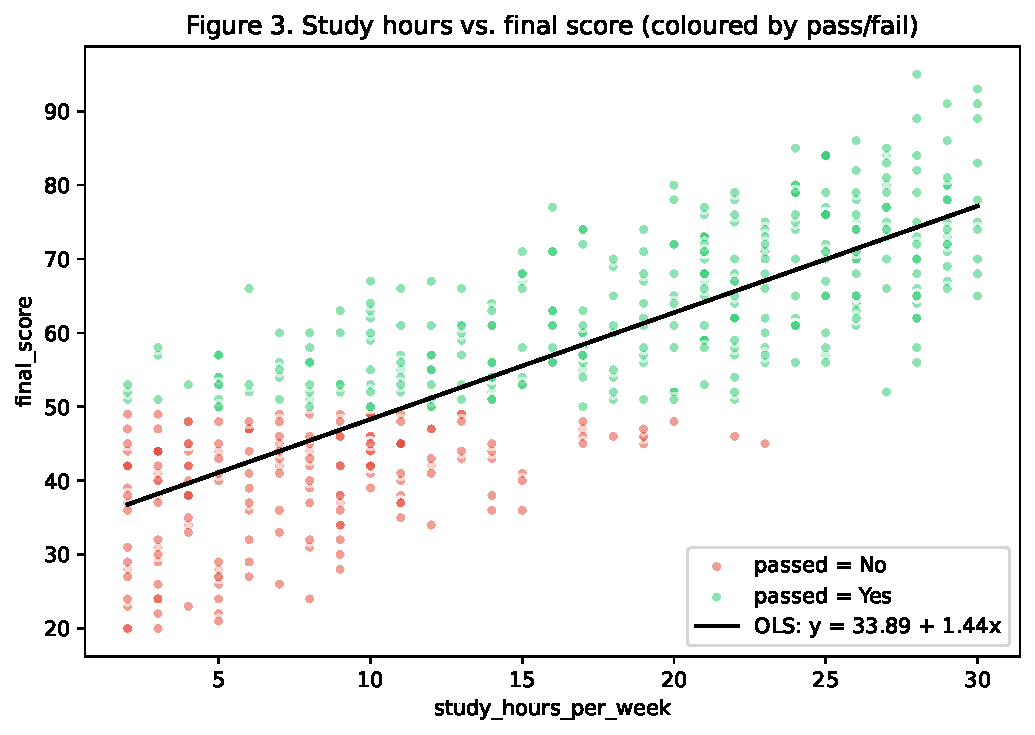
\includegraphics[width=0.75\textwidth]{fig3_hours_vs_score.pdf}
  \caption{Study hours per week vs.\ final score, coloured by pass/fail. The black line is the OLS fit.}
  \label{fig:hours}
\end{figure}

\subsection{Multiple regression on final score}
The OLS model explains 76.7\% of the variance in final score ($R^2=0.767$, Adj.\ $R^2=0.763$, RMSE $=7.49$, $n=500$). Coefficients are summarized in Table~\ref{tab:ols}. Only three predictors are statistically significant at $p<0.05$: study hours, attendance rate, and previous score. All demographic and contextual predictors have $p>0.1$ and standardized effects near zero.

\begin{table}[htbp]
\centering
\small
\caption{OLS regression of \texttt{final\_score} on nine predictors. $R^2=0.767$, Adj.\ $R^2=0.763$, RMSE $=7.49$.}
\label{tab:ols}
\begin{tabular}{lrrrrr}
\toprule
Variable & Coef.\ & SE & $t$ & $p$ & $\beta_{\text{std}}$ \\
\midrule
(Intercept)             & $-3.275$ & $4.829$ & $-0.68$ & $0.498$ & --- \\
study\_hours\_per\_week & $+1.486$ & $0.039$ & $+37.66$ & $<10^{-100}$ & $+0.828$ \\
attendance\_rate        & $+0.293$ & $0.024$ & $+12.00$ & $<10^{-28}$  & $+0.263$ \\
previous\_score         & $+0.194$ & $0.018$ & $+10.82$ & $<10^{-24}$  & $+0.239$ \\
age                     & $+0.173$ & $0.238$ & $+0.73$  & $0.467$      & $+0.016$ \\
internet\_access        & $-0.058$ & $0.675$ & $-0.09$  & $0.932$      & $-0.002$ \\
extracurricular         & $+0.160$ & $0.674$ & $+0.24$  & $0.813$      & $+0.005$ \\
gender (Female)         & $-0.424$ & $0.674$ & $-0.63$  & $0.530$      & $-0.014$ \\
parent\_edu (ordinal)   & $-0.299$ & $0.348$ & $-0.86$  & $0.391$      & $-0.019$ \\
parent\_edu\_missing    & $-0.598$ & $0.816$ & $-0.73$  & $0.464$      & $-0.016$ \\
\bottomrule
\end{tabular}
\end{table}

\begin{figure}[htbp]
  \centering
  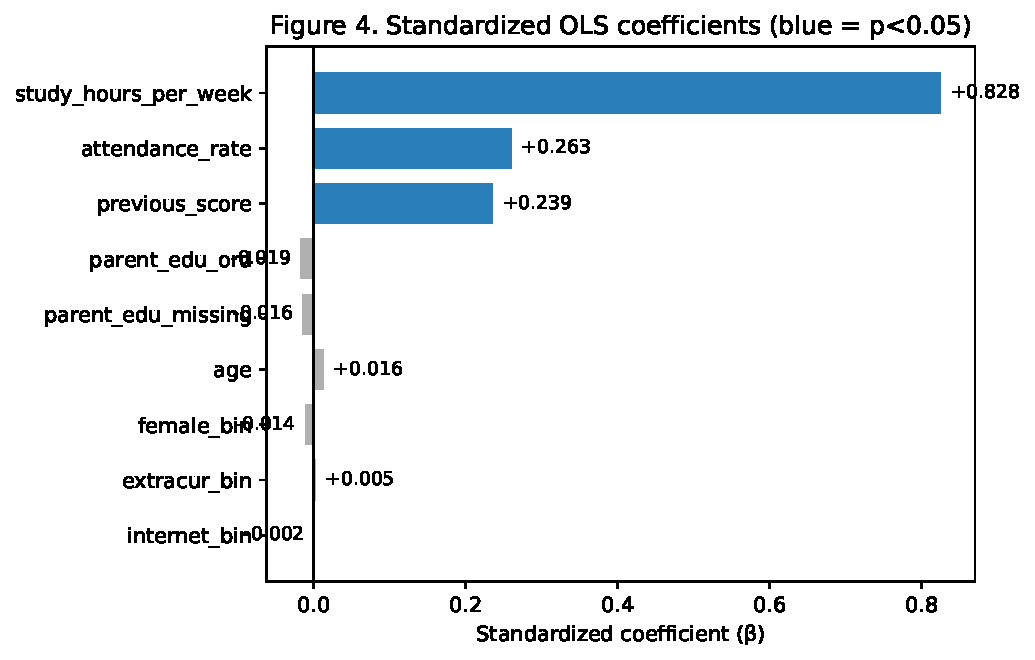
\includegraphics[width=0.8\textwidth]{fig4_std_coefs.pdf}
  \caption{Standardized OLS coefficients. Blue bars: $p<0.05$; grey bars: not significant.}
  \label{fig:stdcoef}
\end{figure}

\subsection{Logistic model for pass/fail}
A logistic regression on the same predictor set classifies pass/fail with 84.4\% accuracy (vs.\ a 64.6\% base rate). The coefficients (Table~\ref{tab:logit}) replicate the OLS pattern: only study hours, attendance, and previous score are significant.

\begin{table}[htbp]
\centering
\small
\caption{Logistic regression of \texttt{passed} on nine predictors. Accuracy $=0.844$ at the 0.5 threshold.}
\label{tab:logit}
\begin{tabular}{lrrrr}
\toprule
Variable & Coef.\ & Odds ratio & $z$ & $p$ \\
\midrule
(Intercept)             & $-12.513$ & --- & $-5.29$ & $1.2\times10^{-7}$ \\
study\_hours\_per\_week & $+0.348$ & $1.42$ & $+10.73$ & $<10^{-25}$ \\
attendance\_rate        & $+0.063$ & $1.07$ & $+5.34$  & $9.1\times10^{-8}$ \\
previous\_score         & $+0.056$ & $1.06$ & $+6.13$  & $8.8\times10^{-10}$ \\
age                     & $+0.064$ & $1.07$ & $+0.63$  & $0.529$ \\
internet\_access        & $-0.334$ & $0.72$ & $-1.13$  & $0.259$ \\
extracurricular         & $+0.021$ & $1.02$ & $+0.07$  & $0.943$ \\
gender (Female)         & $-0.016$ & $0.98$ & $-0.06$  & $0.956$ \\
parent\_edu (ordinal)   & $-0.227$ & $0.80$ & $-1.46$  & $0.144$ \\
parent\_edu\_missing    & $+0.002$ & $1.00$ & $+0.00$  & $0.996$ \\
\bottomrule
\end{tabular}
\end{table}

\subsection{Demographic group comparisons}
Univariate comparisons of final score across demographic and contextual groups show no statistically significant differences:
\begin{itemize}
  \item \textbf{Gender:} Female mean $=55.54$ ($n=273$) vs.\ Male mean $=56.51$ ($n=227$), $t=-0.70$, $p=0.482$.
  \item \textbf{Internet access:} No mean $=55.19$ ($n=246$) vs.\ Yes mean $=56.74$ ($n=254$), $t=-1.13$, $p=0.259$.
  \item \textbf{Extracurricular:} No mean $=55.54$ ($n=253$) vs.\ Yes mean $=56.43$ ($n=247$), $t=-0.65$, $p=0.519$.
  \item \textbf{Parental education:} one-way ANOVA $F(3,379)=2.51$, $p=0.058$.
\end{itemize}

Figure~\ref{fig:parent} shows the distribution of final score by parental education, confirming substantial within-group overlap.

\begin{figure}[htbp]
  \centering
  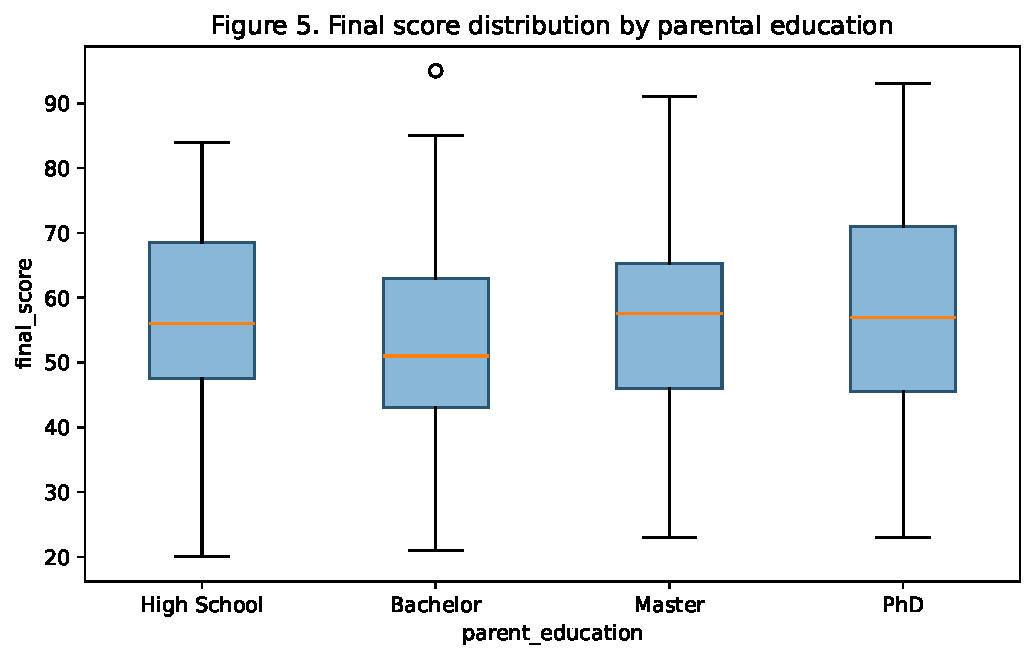
\includegraphics[width=0.7\textwidth]{fig5_parent_edu_box.pdf}
  \caption{Final score by parental education level. Differences across levels are small relative to within-level variance.}
  \label{fig:parent}
\end{figure}

\subsection{Practical translation: pass rate by study-hours tertile}
To translate the study-hours effect into a practical quantity, we grouped students into tertiles of weekly study hours and computed pass rate per tertile (Figure~\ref{fig:tertile}). The pass-rate gap between the top and bottom tertiles is large, underscoring the practical importance of this single variable.

\begin{figure}[htbp]
  \centering
  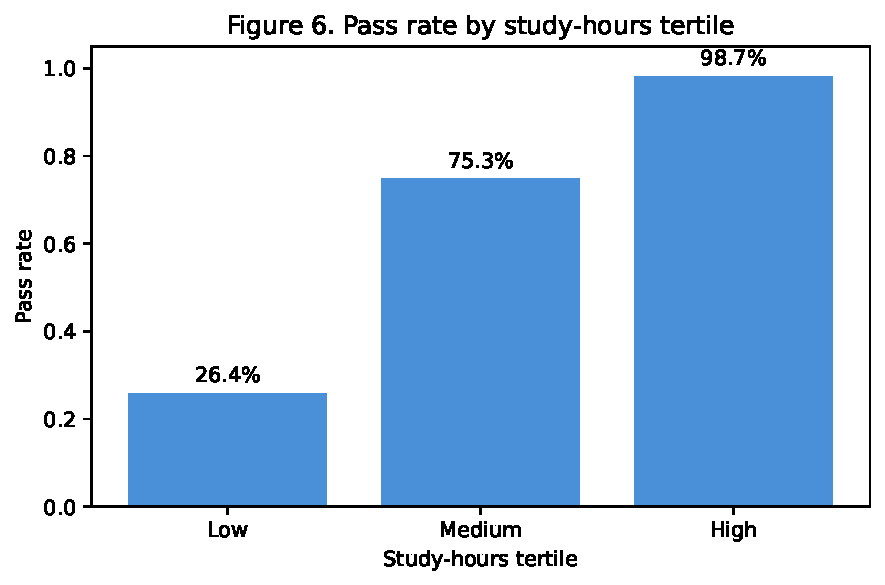
\includegraphics[width=0.65\textwidth]{fig6_pass_by_hours.pdf}
  \caption{Pass rate by study-hours tertile.}
  \label{fig:tertile}
\end{figure}

\section{Discussion}
Three observations stand out.

\paragraph{Effort dominates.} Study hours per week is not merely the strongest predictor---it is dramatically stronger than anything else in the dataset, with a standardized coefficient more than three times the next largest and a $t$-statistic above 37. The 76.7\% variance explained by the full model is almost entirely carried by study hours, attendance, and previous score in combination.

\paragraph{Contextual factors do not add explanatory power.} Gender, age, internet access, extracurricular participation, and parental education are individually uncorrelated with final score and jointly non-significant in the multiple regression. In this dataset, achievement does not appear to be stratified by these demographic dimensions once effort is held constant. We note, however, that this does not rule out indirect effects operating \emph{through} effort---for example, if parental education influences study habits, the reduced-form effect of parental education on the score would be captured by the study-hours coefficient.

\paragraph{Previous score is a weaker predictor than expected.} The correlation between \texttt{previous\_score} and \texttt{final\_score} is only $r=0.17$. If \texttt{previous\_score} reflects a stable ability trait, one would expect a stronger correlation. One possibility is that the data are from a context where recent effort can substantially overcome prior standing; another is that the scores are measured on different scales or assessments. The regression result (significant $+0.19$ coefficient) indicates previous score does retain predictive value once effort is controlled, but its modest magnitude deserves note.

\paragraph{Limitations.} The dataset is a single cross-section of 500 students with no information on school, teacher, curriculum, or the scales of the score variables. The \texttt{parent\_education} variable has 23.4\% missingness, which we handled by median imputation with a missingness indicator; this may attenuate its apparent effect. We did not address potential endogeneity between effort and prior ability, nor interactions between predictors. The generalizability of the findings beyond the sampled population is unknown.

\section{Conclusion}
Weekly study hours and class attendance are the dominant predictors of student final score in this dataset, jointly accounting for the large majority of the 76.7\% variance explained by our OLS model. Demographic and contextual variables do not add significant explanatory power after controlling for effort. A pass/fail classifier built on the same predictors achieves 84.4\% accuracy. The practical implication is clear: in this population, interventions that increase time-on-task and attendance are likely to be the highest-leverage levers for improving academic outcomes, and there is no evidence of demographic achievement gaps conditional on effort.

Future work should extend this analysis with longitudinal data, richer measures of instructional context, and causal identification strategies (e.g., instrumental variables or randomized interventions on study habits) to distinguish the causal from the merely predictive role of effort.

\end{document}
